\subsection{Component view}
In this section, components are expanded and better analyzed. \\
The main analysis regards the microservices block: 
\begin{figure}[H]
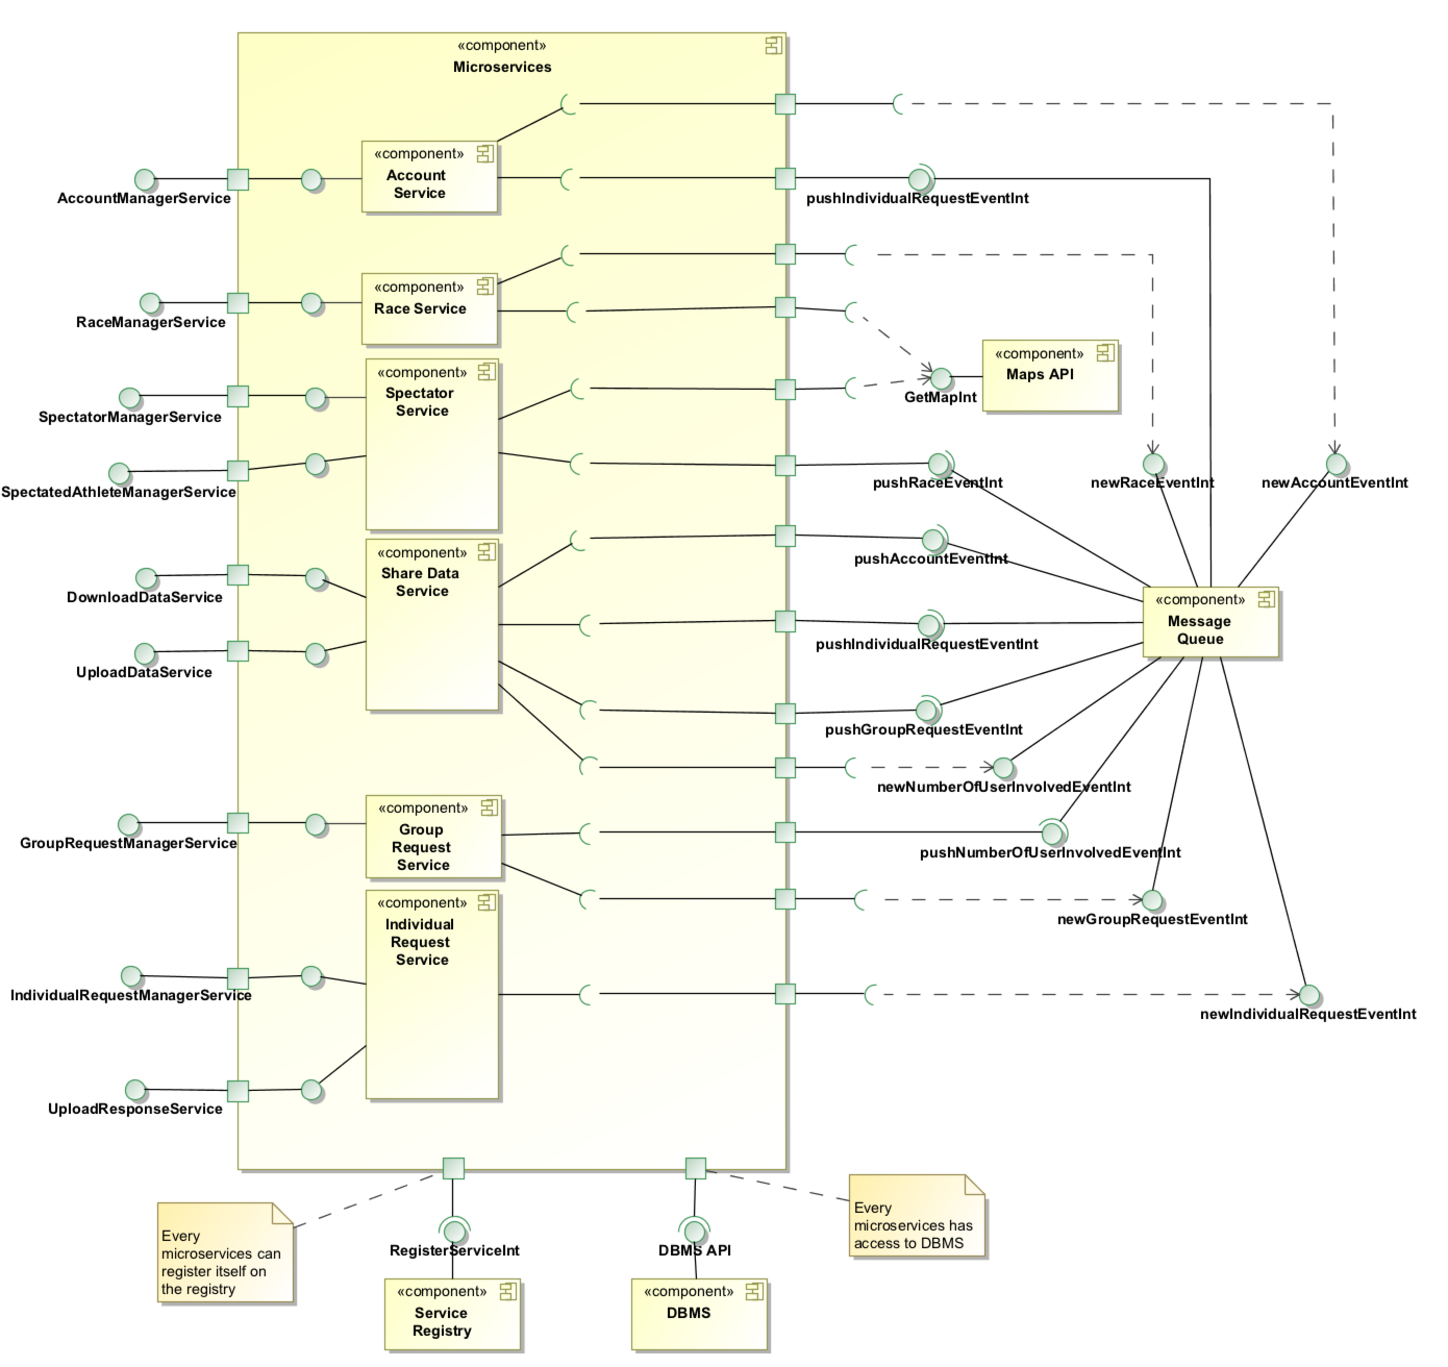
\includegraphics[width=\linewidth]{Images/componentdiagram.pdf}
\caption{ Component diagram }
\label{fig:componentdiagram}
\end{figure}
Various service components are present, and they all expose at least an interface that is accessed by the
clients via the joint combination of API gateway and router.
It follows a brief description of the various services, and a better specification of the interfaces they provide to users and third party customers:
\begin{itemize}
\item The account service provides all the functions related to user sessions, such as login and logout,
and also the registration of clients 
\item The race service makes possible for an athlete to enroll in a run; for a third party customer to set
up one, and also close it; and it also enables the possibility of retrieving the available races and their
status (e.g. in course, terminated). Therefore, it manages the "more static" part
of a race
\item The spectator service regards the dynamic part of a race, such as the fact that a user can spectate
athletes who are running (therefore they can retrieve their positions and the leaderboard). This
service is also in charge of receiving position data of the participants
\item Share data service is responsible for the monitoring the user health statuses and positions: here a
user will upload his data. Furthermore, third party customer will access the data that they have
previously requested, by means of "AccessDataService" interface
\item The group request service provides to the third parties the possibility of uploading group requests and see their status 
\item The individual request service enables third party customer to upload individual request and monitor their status, and allows a user to
check if there are some requests for him, and, eventually, upload responses 
\end{itemize}

Microservices have their own data and, therefore, access DBMS's API, while Maps's API are necessary 
only for race and spectator service, in order to manage and double check position data and feasible paths. \\
The diagram also shows the main communications that take place between components. 
The following message exchange is needed to completely and correctly exploit the project functions. 
\begin{itemize}
\item 
When a third party is accessing individual data through the data share service, it
needs to know if a request associated with those data was sent and accepted. 
Indeed, the request acceptance and its data, are managed in the following way: when an individual request has been accepted, a message is sent through the message queue with the help of an interface, IndividualRequestEventPublisher. Then, this message reaches the share data service thanks to the interface provided by it (i.e. IndividualRequestEventListener). \\
Moreover, to guarantee that individual requests must be performed on registered users, a match with the account service 
is necessary. When a new user registers, the account service will send the data about the user through the message queue to reach 
all the services which need it. One of these services is the Individual Request Service which needs the user to check if an individual 
request is coherent with the system (UserEventListener and UserEventPublisher are the interfaces that accomplish this task). 
\item 
A slightly different reasoning holds for the management of the group requests. In this case, the exchange is bidirectional. 
In particular, when a new group request is performed, the share data service will be notified by the message queue via the
GroupRequestEventListener, and it will be sent to the message queue by GroupRequestEventPublisher. \\
When the share data service receives this event, it will query its data in order to retrieve information regarding the number of users
involved: of course, this information needs to be sent back to the group request service, that will accept or refuse the request
(DataEventListener and DataEventPublisher are the interfaces that accomplish this task). 
Of course, the acceptance of the request may trigger again the new group request event. 
However, this will be later exposed and commented in the run time view. \\
Moreover, to guarantee that the filters on the aggregated request are applied correctly (e.g. data on the users whose age is greater then 40)
a match with the account service is needed. 
Indeed, when a user registers to the service, the account service will sends user information to the message queue with UserEventPublisher. 
The information will be forwarded to the share data service with UserEventListener.
\item
Another important message exchange is between spectator and race services: in particular, data that the spectator service is receiving must
be matched with an active run, and thus it needs to know the status of the run: the changes will be communicated by 
RaceEventListener and RaceEventPublisher.
\end{itemize}
